% Atomic energy level diagram — pure TikZ (hand-placed).
% For a diagram with more than ~4 levels use the generator instead:
%   python3 $LUXAS_ROOT/skills/figure/scripts/levelspec <name>.levelspec.json
% (compressed energy axis, straight drives / wavy decays, labels in slots, no key box).
\documentclass[border=4pt]{standalone}
\usepackage{tikz}
\usepackage{amsmath}
\usepackage{braket}
\usetikzlibrary{arrows.meta,decorations.pathmorphing}

\definecolor{atomC}{HTML}{0072B2}
\definecolor{ionC}{HTML}{D55E00}

\begin{document}
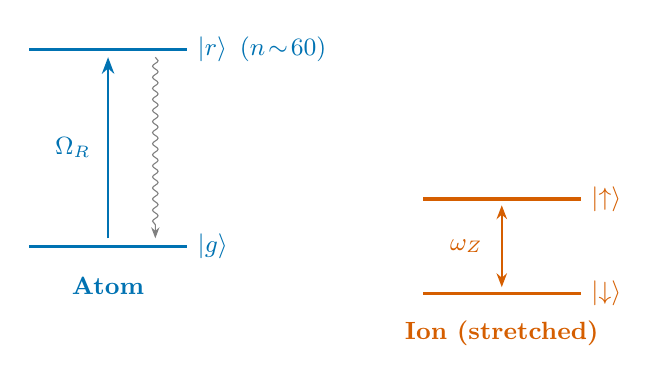
\begin{tikzpicture}[font=\sffamily]

  % Ground + Rydberg pair (atom)
  \draw[atomC, very thick] (0,0)    -- (2.0, 0)    node[right,font=\small]{$\ket{g}$};
  \draw[atomC, very thick] (0,2.5)  -- (2.0, 2.5)  node[right,font=\small]{$\ket{r}\ (n\!\sim\!60)$};
  % Laser drive: a STRAIGHT arrow. Convention: straight = coherent drive (laser,
  % microwave), wavy (snake) = spontaneous emission / decay. The Ba run
  % (2026-08-30) drew every laser wavy because this template did.
  \draw[atomC, thick, -{Stealth[length=6pt]}] (1.0, 0.1) -- (1.0, 2.4);
  % Decay back to the ground state: wavy, thin, grey.
  \draw[gray, thin, decorate, decoration={snake, amplitude=1.0pt, segment length=4pt, post length=4pt},
        -{Stealth[length=4pt]}] (1.6, 2.4) -- (1.6, 0.1);
  \node[atomC, font=\small\itshape] at (0.55, 1.25) {$\Omega_R$};
  \node[atomC, font=\small\bfseries] at (1.0, -0.5) {Atom};

  % Zeeman stretched (ion)
  \begin{scope}[xshift=5cm]
    \draw[ionC, very thick] (0,  0.6) -- (2.0, 0.6) node[right,font=\small]{$\ket{\uparrow}$};
    \draw[ionC, very thick] (0, -0.6) -- (2.0,-0.6) node[right,font=\small]{$\ket{\downarrow}$};
    \draw[ionC, thick, {Stealth[length=5pt]}-{Stealth[length=5pt]}] (1.0, 0.52) -- (1.0, -0.52);
    \node[ionC, font=\small\itshape] at (0.55, 0) {$\omega_Z$};
    \node[ionC, font=\small\bfseries] at (1.0, -1.1) {Ion (stretched)};
  \end{scope}

\end{tikzpicture}
\end{document}
